\section{Ejercicio 6}

$$
F(w,x,y,z) = \sum(2,3,12,13,14,15)\; , \; X = 6,7,10,11
$$

\subsection{Expresión mínima}

\begin{figure}[H]
    \centering
    \begin{karnaugh-map}[4][4][1][$z$][$y$][$x$][$w$]
        \minterms{2,3,12,13,14,15}
        \terms{6,7,10,11}{X}
        \implicant{3}{10}
        \implicant{12}{14}
    \end{karnaugh-map}
    \caption{Mapa de Karnaugh para la función}
\end{figure}

$$
F(w,x,y,z) = wx + y
$$

\subsection{Simulación en Falstad}
\begin{figure}[H]
    \centering
    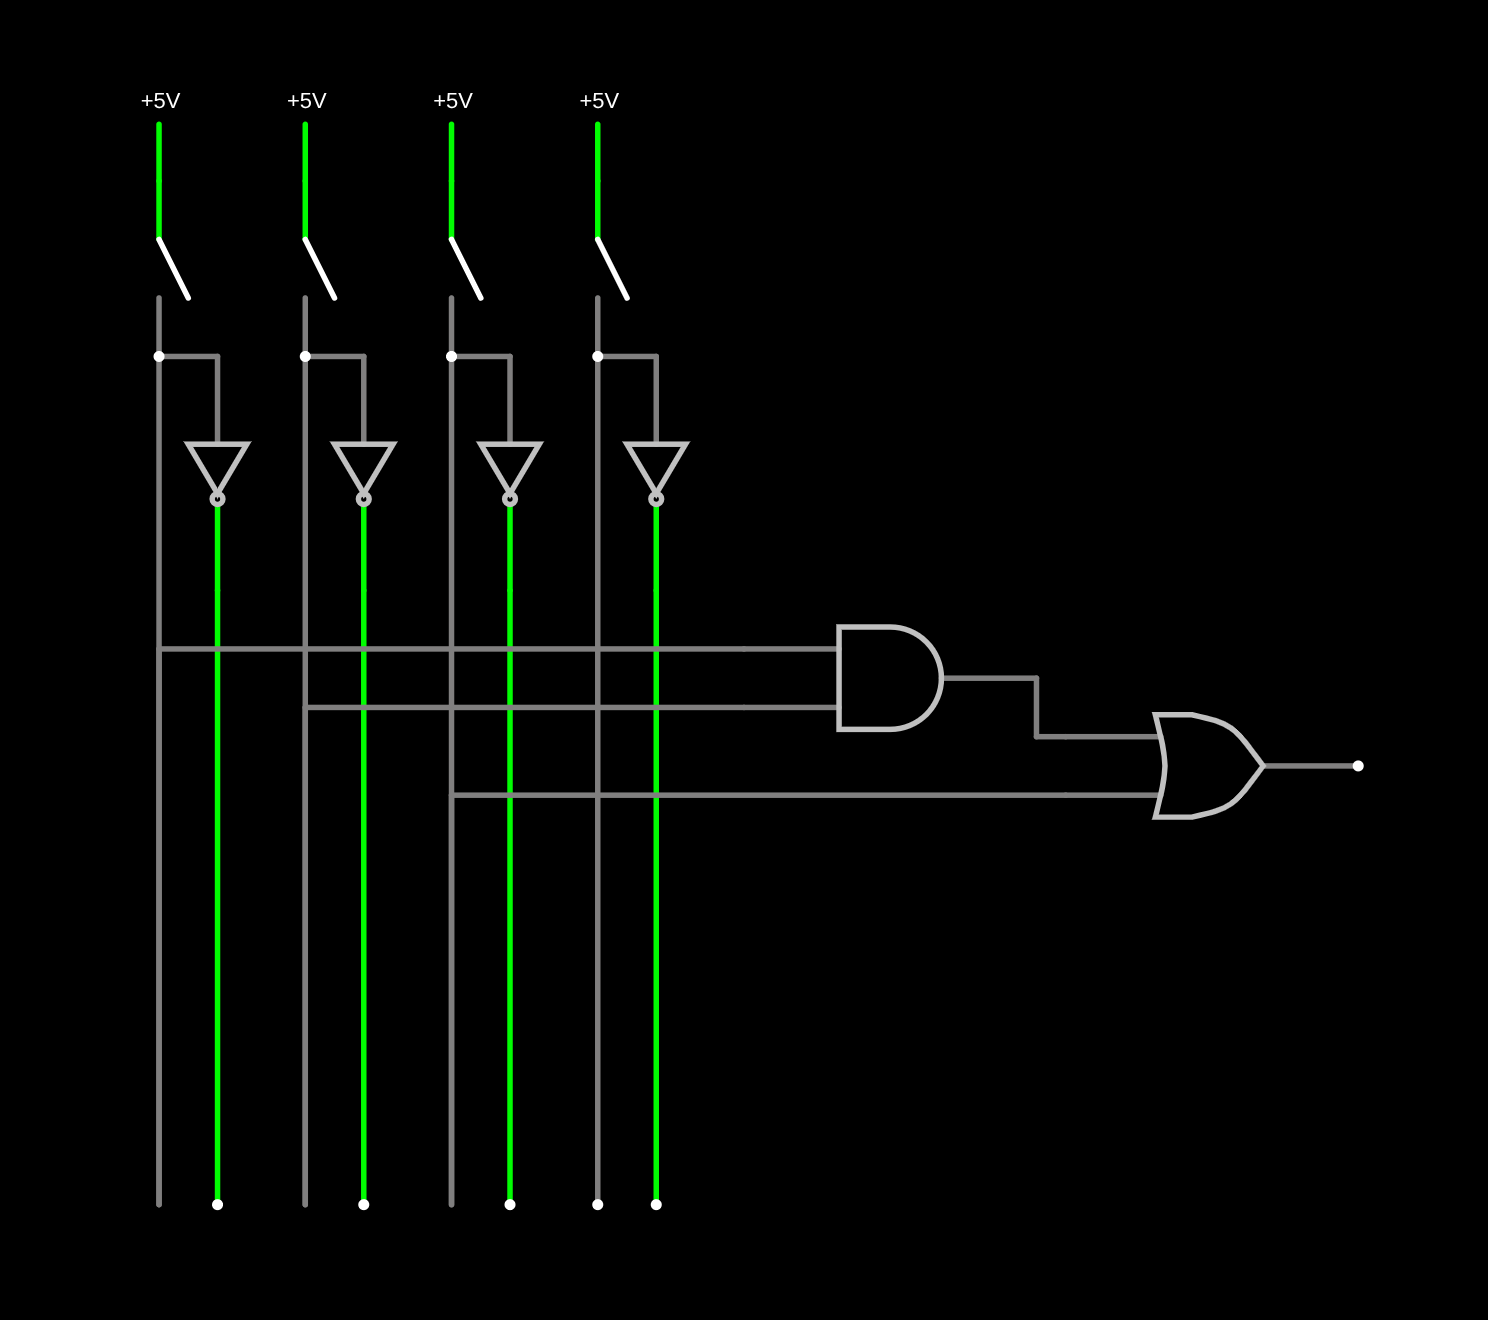
\includegraphics[width=0.6\textwidth]{img/Falstad/ej6.png}
    \caption{Simulación de la función en Falstad}
\end{figure}

\subsection{Descripción en Verilog}

\begin{Verbatim}[ frame=single, fontsize=\small, baselinestretch=1.2 ]
module ej6 (
    input w,
    input x,
    input y,
    input z,
    output F
);

assign F = w&x | y;

endmodule
\end{Verbatim}

\subsection{Captura del RTL}
\begin{figure}[H]
    \centering
    
\includegraphics[width=0.8\textwidth]{img/Xilinx/ej6.png}
    \caption{Captura del RTL en Xilinx}
\end{figure}